\let\negmedspace\undefined
\let\negthickspace\undefined
\documentclass[journal]{IEEEtran}
\usepackage[a5paper, margin=10mm, onecolumn]{geometry}
\usepackage{lmodern} % Ensure lmodern is loaded for pdflatex
\usepackage{tfrupee} % Include tfrupee package

\setlength{\headheight}{1cm} % Set the height of the header box
\setlength{\headsep}{0mm}     % Set the distance between the header box and the top of the text

\usepackage{gvv-book}
\usepackage{gvv}
\usepackage{cite}
\usepackage{amsmath,amssymb,amsfonts,amsthm}
\usepackage{algorithmic}
\usepackage{graphicx}
\usepackage{textcomp}
\usepackage{xcolor}
\usepackage{txfonts}
\usepackage{listings}
\usepackage{enumitem}
\usepackage{mathtools}
\usepackage{gensymb}
\usepackage{comment}
\usepackage[breaklinks=true]{hyperref}
\usepackage{tkz-euclide} 
\usepackage{listings}
\usepackage{gvv}                                        
\def\inputGnumericTable{}                                 
\usepackage[latin1]{inputenc}                                
\usepackage{color}                                            
\usepackage{array}                                            
\usepackage{longtable}                                       
\usepackage{calc}                                             
\usepackage{multirow}                                         
\usepackage{hhline}                                           
\usepackage{ifthen}                                           
\usepackage{lscape}
\begin{document}

\bibliographystyle{IEEEtran}
\vspace{3cm}

\title{NCERT-8.2.7}
\author{EE24BTECH11036 - Krishna Patil}
% \maketitle
% \newpage
% \bigskip
{\let\newpage\relax\maketitle}
\renewcommand{\thefigure}{\theenumi}
\renewcommand{\thetable}{\theenumi}
\setlength{\intextsep}{10pt} % Space between text and floats

\textbf{Question : } Calculate the area bounded by the curves $y^2 = 4x$ and $y = 2x$ . \\
\solution \\
\textbf{(a) Theoretical Solution : }
\begin{enumerate}
    \item \textbf{Find Points of Intersection:} \\  
\item \textbf{Find Points of Intersection:} \\  
    For \( y^2 = 4x \):
    \[
    V_1 = \myvec{ 
    0 & 0 \\ 
    0 & 1 
    }, \quad 
    u_1 = \myvec{ 
    -2 \\ 
    0 
    }, \quad 
    f_1 = 0
    \]
    The quadratic form is:
    \[
    \myvec{ 
    x \\ 
    y 
    }^\top 
    \myvec{ 
    0 & 0 \\ 
    0 & 1 
    }
    \myvec{ 
    x \\ 
    y 
    }
    + 2 \myvec{ 
    -2 & 0 
    }
    \myvec{ 
    x \\ 
    y 
    }
    + 0 = 0
    \]

    For \( y = 2x \):
    \[
    V_2 = \myvec{ 
    0 & 0 \\ 
    0 & 0 
    }, \quad 
    u_2 = \myvec{ 
    -1 \\ 
    0.5 
    }, \quad 
    f_2 = 0
    \]
    The quadratic form is:
    \[
    \myvec{ 
    x \\ 
    y 
    }^\top 
    \myvec{ 
    0 & 0 \\ 
    0 & 0 
    }
    \myvec{ 
    x \\ 
    y 
    }
    + 2 \myvec{ 
    -1 & 0.5 
    }
    \myvec{ 
    x \\ 
    y 
    }
    + 0 = 0
    \]

    \item \textbf{Write the two equations in matrix form:}
    \begin{itemize}
        \item From \( Q_1(x, y) \):
        \[
        \myvec{ 
        x \\ 
        y 
        }^\top 
        \myvec{ 
        0 & 0 \\ 
        0 & 1 
        }
        \myvec{ 
        x \\ 
        y 
        }
        + 2 \myvec{ 
        -2 \\ 
        0 
        }^\top 
        \myvec{ 
        x \\ 
        y 
        }
        = 0
        \]
        Simplifies to:
        \[
        y^2 - 4x = 0
        \]

        \item From \( Q_2(x, y) \):
        \[
        2 \myvec{ 
        -1 \\ 
        0.5 
        }^\top 
        \myvec{ 
        x \\ 
        y 
        }
        = 0
        \]
        Simplifies to:
        \[
        -2x + y = 0 \quad \text{or equivalently, } y = 2x
        \]
    \end{itemize}

    \item \textbf{Substitute \( y = 2x \) from \( Q_2(x, y) \) into \( Q_1(x, y) \):}
    \begin{align}
    (2x)^2 - 4x &= 0 \\
    4x^2 - 4x &= 0 \\
    x(x - 1) &= 0
    \end{align}

    \item \textbf{Solve for \( x \):}
    \[
    x = 0 \quad \text{or} \quad x = 1
    \]

    \item \textbf{Find \( y \) for each \( x \):}
    \begin{itemize}
        \item For \( x = 0 \), \( y = 2(0) = 0 \)
        \item For \( x = 1 \), \( y = 2(1) = 2 \)
    \end{itemize}

    \item \textbf{The intersection points are:}
    \[
    (0, 0) \quad \text{and} \quad (1, 2)
    \]


    \item \textbf{Set Up the Integral:}  \\
    The parabola is $y^2 = 4x \implies x = \frac{y^2}{4}$, and the line is $x = \frac{y}{2}$.  
    To calculate the area, we integrate the difference between the parabola and the line in terms of $y$, from $y = 0$ to $y = 2$:
    \begin{align}
        \text{Area} = \int_{y=0}^{y=2} \brak{ \frac{y}{2} - \frac{y^2}{4} } \, dy.
    \end{align} \\

    \item \textbf{Evaluate the Integral:}  \\
    Expand the integral:
    \begin{align}
        \text{Area} = \int_{0}^{2} \frac{y}{2} \, dy - \int_{0}^{2} \frac{y^2}{4} \, dy.
    \end{align}

    First term:
    \begin{align}
        \int_{0}^{2} \frac{y}{2} \, dy &= \frac{1}{2} \int_{0}^{2} y \, dy = \frac{1}{2} \brak{ \frac{y^2}{2} }_{0}^{2} = \frac{1}{2} \cdot \frac{4}{2} = 1.
    \end{align}

    Second term:
    \begin{align}
        \int_{0}^{2} \frac{y^2}{4} \, dy &= \frac{1}{4} \int_{0}^{2} y^2 \, dy = \frac{1}{4} \brak{ \frac{y^3}{3} }_{0}^{2} = \frac{1}{4} \cdot \frac{8}{3} = \frac{2}{3}.
    \end{align}

    Now subtract:
    \begin{align}
        \text{Area} = 1 - \frac{2}{3} = \frac{3}{3} - \frac{2}{3} = \frac{1}{3}.
    \end{align} \\
    
\textbf{(b) Numerical Solution / Simulation : } \\

We aim to compute the integral:

\[
I = \int_0^2 \left( \frac{y}{2} - \frac{y^2}{4} \right) \, dy
\]

using the trapzoidal trule approach. \\

    \item \textbf{Discretize the Interval:}  
    Divide the interval $[0, 2]$ into $N = 100$ equal subintervals. The step size is:
    \begin{align}
    h = \frac{2 - 0}{N} = \frac{2}{100} = 0.02.
    \end{align}
    The discrete points are:
    \begin{align}
    y_i = 0 + i \cdot h, \quad \text{for } i = 0, 1, 2, \dots, 100.
    \end{align}
    For example:
    \begin{align}
    y_0 = 0, \quad y_1 = 0.02, \quad y_2 = 0.04, \, \dots, \, y_{100} = 2.
    \end{align}

    \item \textbf{Define the Function:}  
    The function to integrate is:
    \begin{align}
    f(y) = \frac{y}{2} - \frac{y^2}{4}.
    \end{align} \\

    \item \textbf{Establish the difference equation:} 
    
    Using the trapazoidal rule , 
    \begin{align}
    I_{n} = I_{n-1} + \frac{h}{2} \brak{ f(y_n) + f(y_{n-1})} 
      \end{align}
    where:
    \begin{enumerate}
        \item $I_n$: The approximate integral value up to the $n$-th point,
        \item $h = 0.02$: The step size,
        \item $f\brak{y_n} = \frac{y_n}{2} - \frac{y_n^2}{4}$: The function evaluated at $y_n$. \\
    \end{enumerate} 
   
      So, the integral can be approximated as, 
    \begin{align}
    \label{trap}
    I_n &= I_{n-1} + \frac{h}{2} \brak{ \brak{\frac{y_n}{2} - \frac{y_n^2}{4}} + \brak{\frac{y_{n-1}}{2} - \frac{y_{n-1}^2}{4}}} \\ 
    y_n &= y_{n-1} + h
   \end{align}
    \item \textbf{Iterative Computation:}  
    The recurrence relation is applied iteratively starting with the initial condition:
    \begin{align}
    I_0 = 0.
    \end{align}
    Each step updates $I_n$ using the values of $f(y_n)$ and $f(y_{n-1})$. \\

    \item \textbf{Final Value:}  
    After iterating up to $n = 100$, the value of the integral at the upper bound $y = 2$ is:
    \begin{align}
    I[100] \approx 0.3333
    \end{align}

\textbf {Using the difference equation \eqref{trap} we can code to simulate the area pretty easily . Choosing n = 100 we get area as 0.3333 which verifies with the theoretical solution.}

	 \begin{figure}[h]  % The 'h' means 'here' (positioning)
    \centering  % Centers the figure
    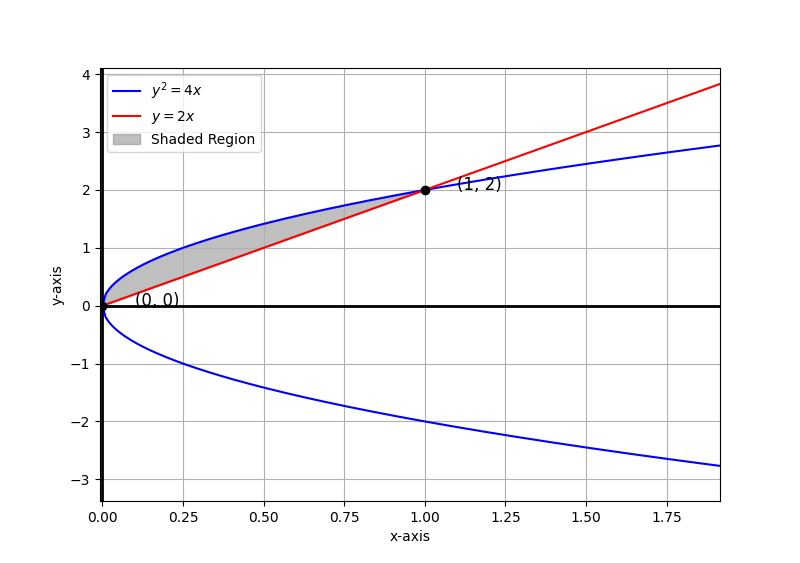
\includegraphics[width=\columnwidth]{fig/Figure_1.png}  
    \caption{Graph}
    \label{fig:example}  % Label for referencing
\end{figure}
\end{enumerate}
\end{document}
